\documentclass{article}

\usepackage[utf8]{inputenc}
\usepackage[french]{babel}

\usepackage{lmodern}
\usepackage{listings}
\usepackage{graphicx}
\usepackage{hyperref}
\usepackage{graphicx}
\usepackage{natbib}
\usepackage{tcolorbox}
\usepackage{xcolor}
\usepackage{array}
\usepackage{pifont}
\usepackage[a4paper, margin=1.5cm]{geometry}  
\usepackage{longtable}
\usepackage{float}
\usepackage{placeins}

\graphicspath{ {./res/} }
\author{
    Valentin Jonquière,
    Mathilde Chollon
}

\title{Rapport Architecture Logicielle}

\begin{document}

\maketitle

\pagebreak

\tableofcontents

\pagebreak

\section{Design patterns utilisés}

\subsection{Prototype}

\subsection{Builder}

\begin{figure}[h]
    \centering
    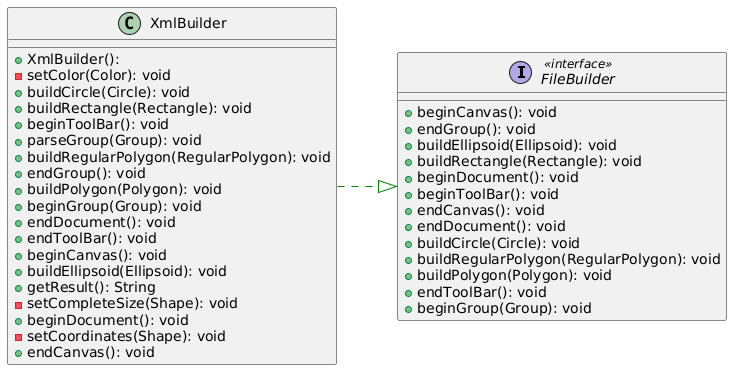
\includegraphics[width=\textwidth,height=5.0cm,keepaspectratio]{builder.png}
    \caption{Diagramme UML du Builder}
    \label{Builder}
\end{figure}
\FloatBarrier


\subsection{Composite}

\begin{figure}[h]
    \centering
    \includegraphics[width=\textwidth,height=15.0cm,keepaspectratio]{Composite.png}
    \caption{Diagramme UML du Composite}
    \label{Composite}
\end{figure}
\FloatBarrier

\subsection{Singleton}

\begin{figure}[h]
    \centering
    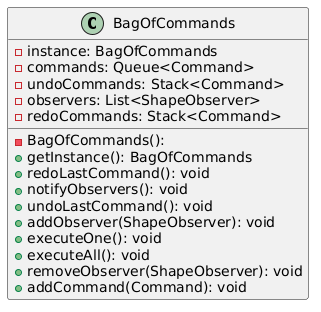
\includegraphics[width=\textwidth,height=5.0cm,keepaspectratio]{singleton.png}
    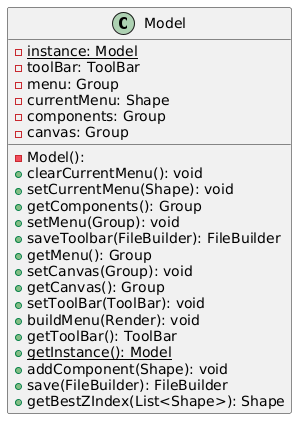
\includegraphics[width=\textwidth,height=5.0cm,keepaspectratio]{singleton2.png}
    \caption{Diagramme UML des deux Singleton}
    \label{Singleton}
\end{figure}
\FloatBarrier

\subsection{Visitor}

\begin{figure}[h]
    \centering
    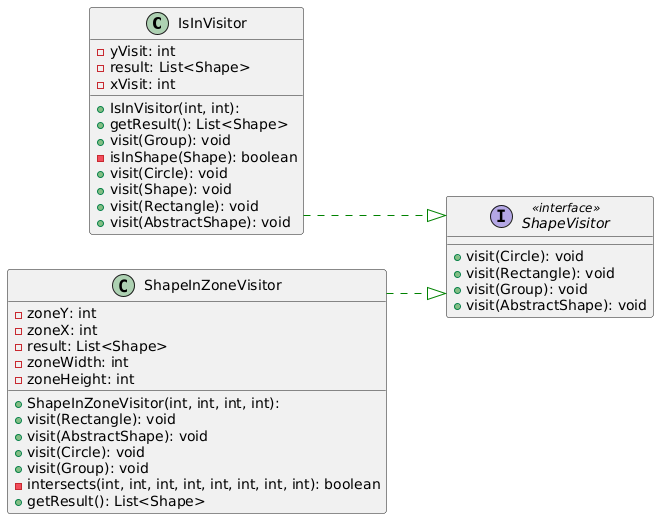
\includegraphics[width=\textwidth,height=10.0cm,keepaspectratio]{visitor.png}
    \caption{Diagramme UML du Visitor}
    \label{Visitor}
\end{figure}
\FloatBarrier
\subsection{Method factory}

\begin{figure}[h]
    \centering
    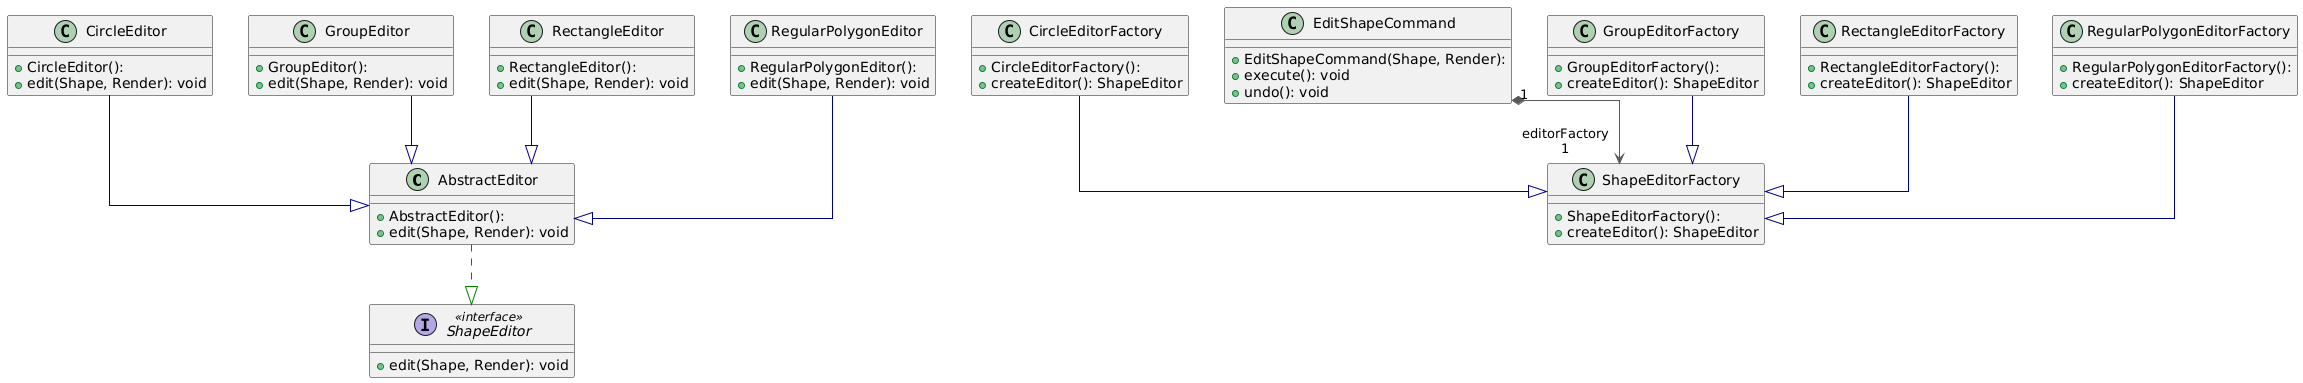
\includegraphics[width=\textwidth,height=10.0cm,keepaspectratio]{methodFactory.png}
    \caption{Diagramme UML de la Method Factory}
    \label{MethodFactory}
\end{figure}
\FloatBarrier
\subsection{Bridge}
\begin{figure}[h]
    \centering
    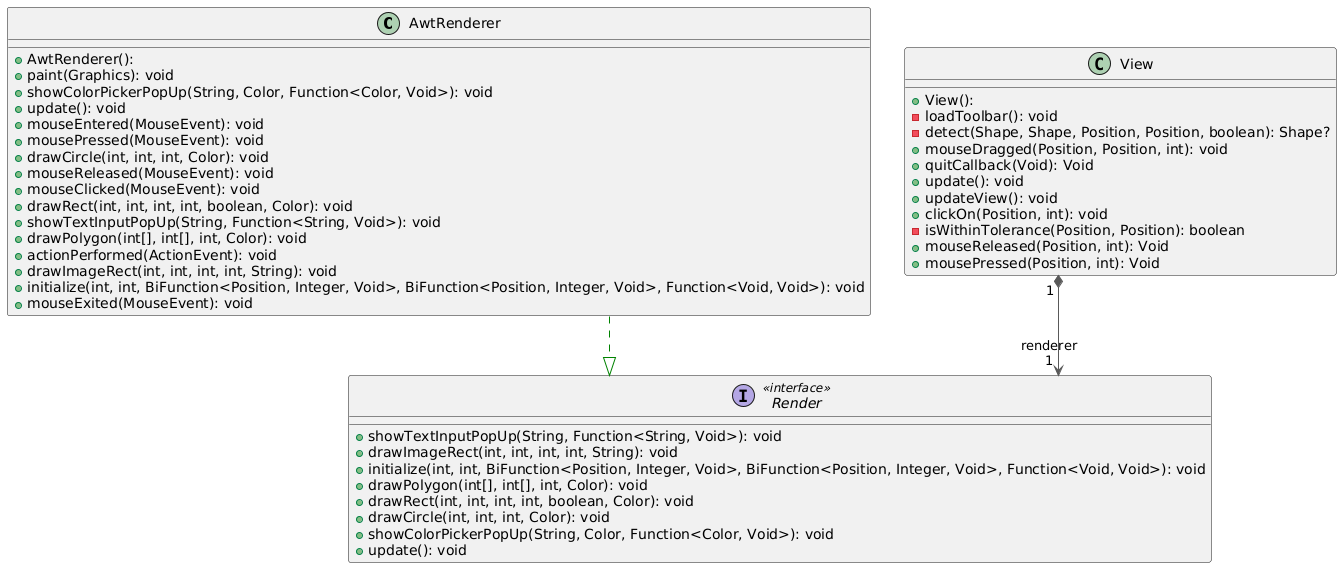
\includegraphics[width=\textwidth,height=10.0cm,keepaspectratio]{bridge.png}
    \caption{Diagramme UML du Bridge}
    \label{Bridge}
\end{figure}
\FloatBarrier
\subsection{Observer}
\begin{figure}[h]
    \centering
    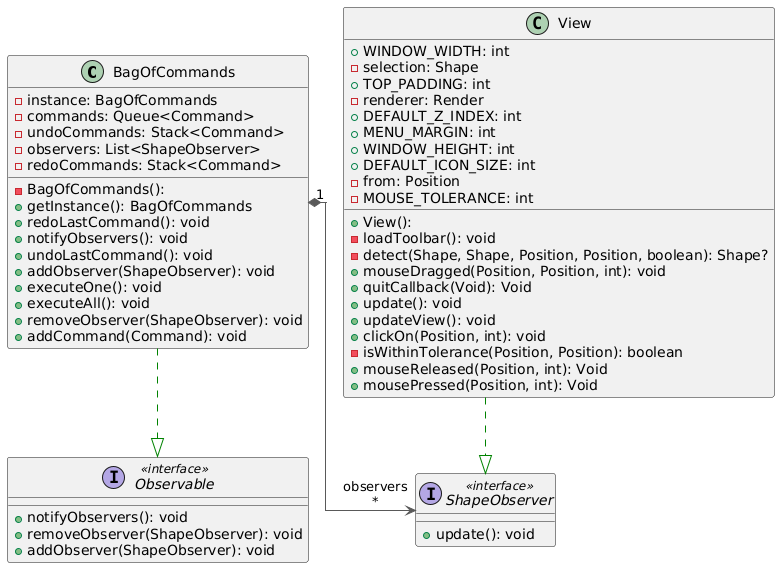
\includegraphics[width=\textwidth,height=10.0cm,keepaspectratio]{observer.png}
    \caption{Diagramme UML de l'Observer}
    \label{Observer}
\end{figure}
\FloatBarrier

\subsection{Memento}
\begin{figure}[h]
    \centering
    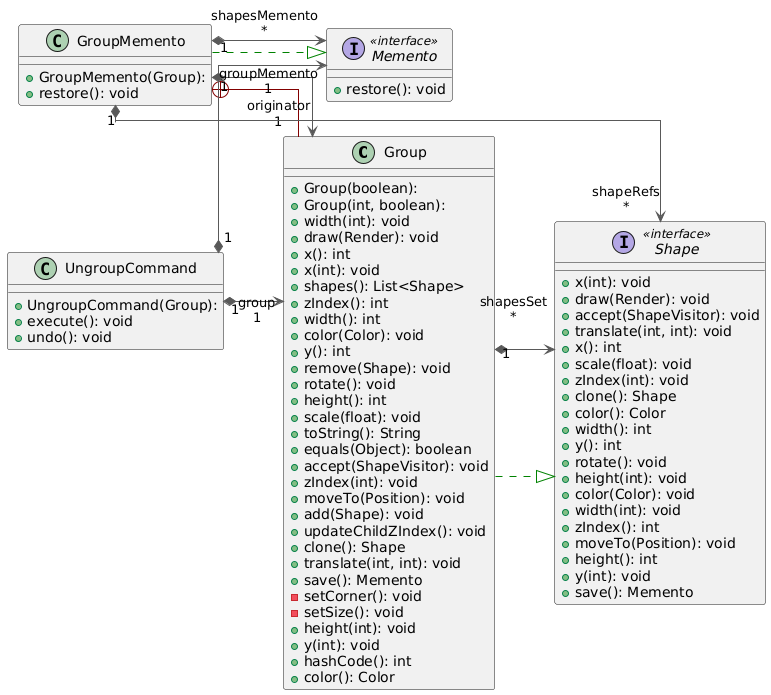
\includegraphics[width=\textwidth,height=10.0cm,keepaspectratio]{memento.png}
    \caption{Diagramme UML du Memento pour un groupe}
    \label{MementoGroupe}
\end{figure}
\FloatBarrier

\begin{figure}[h]
    \centering
    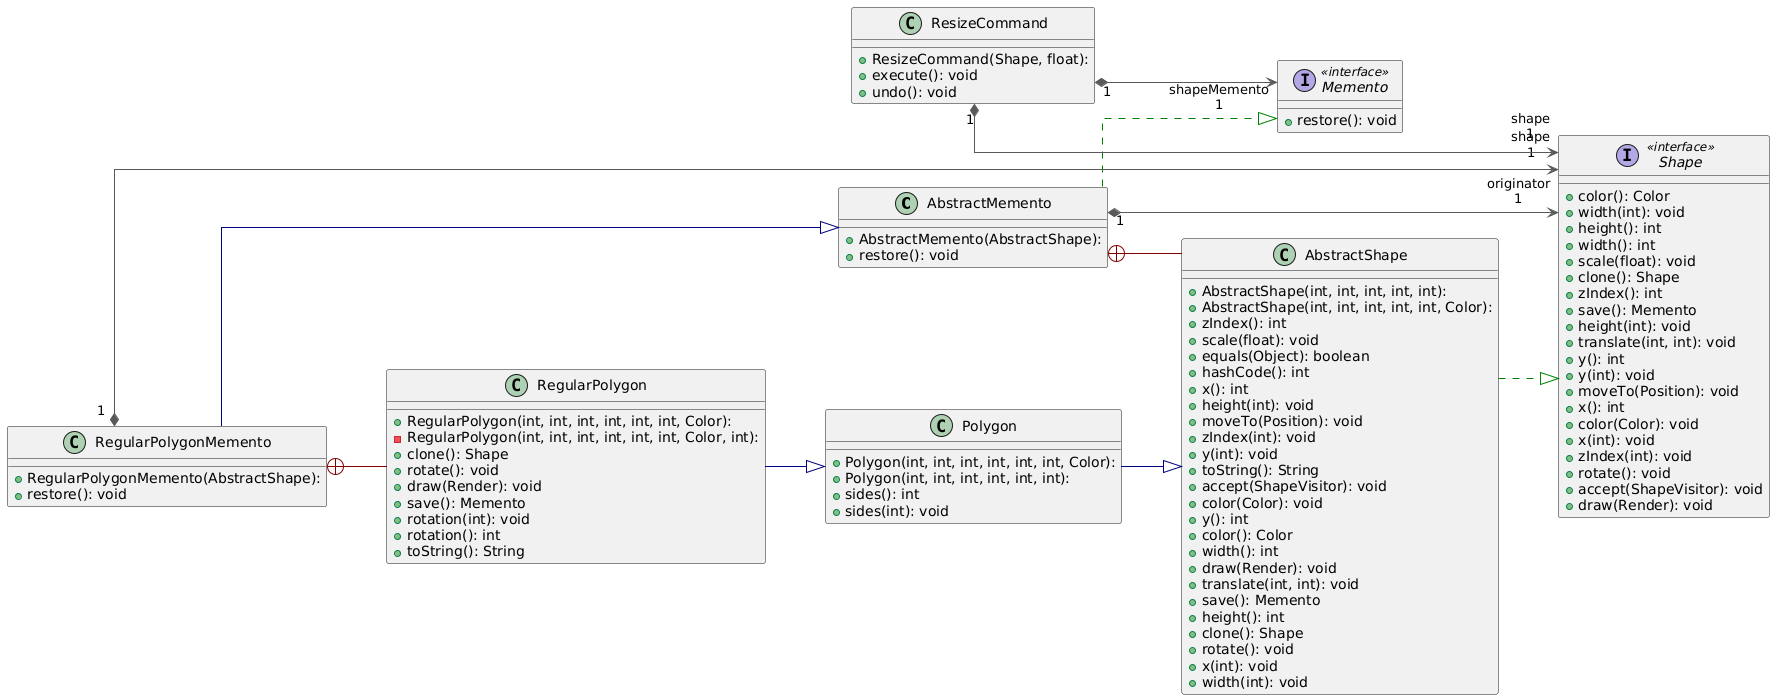
\includegraphics[width=\textwidth,height=10.0cm,keepaspectratio]{memento2.png}
    \caption{Diagramme UML du Memento pour une forme simple}
    \label{MementoShape}
\end{figure}
\FloatBarrier

\subsection{Command + Bag Of Command}

\begin{figure}[h]
    \centering
    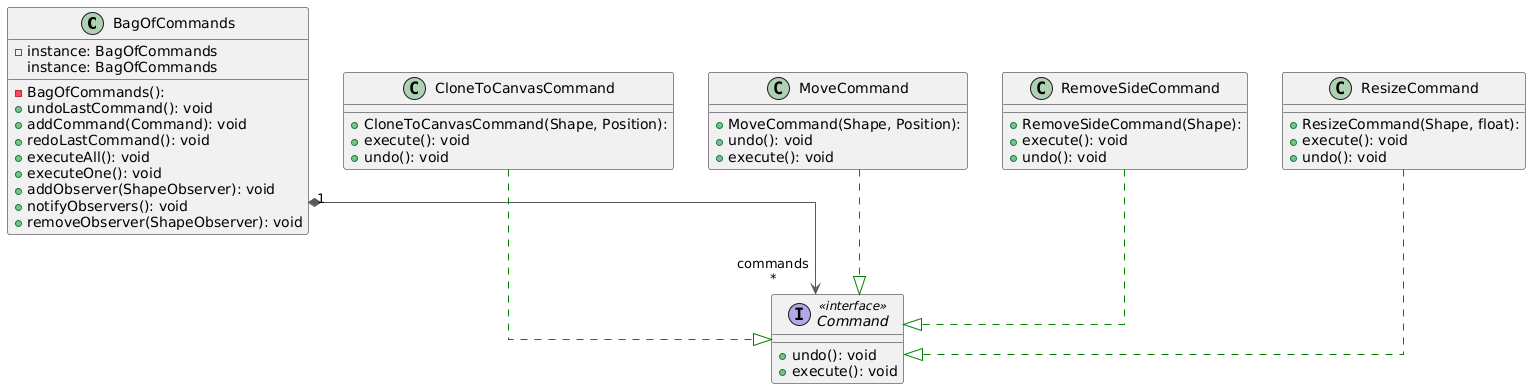
\includegraphics[width=\textwidth,height=10.0cm,keepaspectratio]{command.png}
    \caption{Diagramme UML des Commandes}
    \label{Command}
\end{figure}
\FloatBarrier

\end{document}